\documentclass[12pt, titlepage]{article}

\usepackage{booktabs}
\usepackage{float}
\usepackage{tabularx}
\usepackage{hyperref}
\hypersetup{
    colorlinks,
    citecolor=black,
    filecolor=black,
    linkcolor=red,
    urlcolor=blue
}
\usepackage[round]{natbib}
\usepackage{longtable}
\usepackage[shortlabels]{enumitem}
\usepackage{hyperref}
\hypersetup{
    colorlinks,
    citecolor=blue,
    filecolor=black,
    linkcolor=red,
    urlcolor=blue
}
\usepackage{amsmath}
\usepackage{array}
\usepackage{graphicx}
\usepackage[paper=a4paper]{geometry}

\input{../Comments}
%% Common Parts

\newcommand{\progname}{Room8} % PUT YOUR PROGRAM NAME HERE
\newcommand{\authname}{Team 19
\\ Mohammed Abed
\\ Maged Armanios
\\ Jinal Kasturiarachchi
\\ Jane Klavir
\\ Harshil Patel} % AUTHOR NAMES

\usepackage{hyperref}
    \hypersetup{colorlinks=true, linkcolor=blue, citecolor=blue, filecolor=blue,
                urlcolor=blue, unicode=false}
    \urlstyle{same}
                                


\begin{document}

\title{Verification and Validation Report: Room8} 
\author{\authname}
\date{\today}
	
\maketitle

\pagenumbering{roman}

\section{Revision History}

\begin{tabularx}{\textwidth}{p{3cm}p{2cm}X}
\toprule {\bf Date} & {\bf Version} & {\bf Notes}\\
\midrule
March 10, 2025 & 1 & Authors on front page\\
\bottomrule
\end{tabularx}

~\newpage

\section{Symbols, Abbreviations and Acronyms}

\renewcommand{\arraystretch}{1.2}
\begin{tabular}{l l} 
  \toprule		
  \textbf{Acronym} & \textbf{description}\\
  \midrule 
  SRS & Software Requirements Specification\\
  VnV & Verification and Validation\\
  CI/CD & Continuous Integration and Continuous deployment\\   
  API & Application Programming Interface\\
  Exp. & Expected\\
  Act. & Actual\\
  \bottomrule
\end{tabular}\\


\newpage

\tableofcontents

\listoftables %if appropriate

\listoffigures %if appropriate

\newpage

\pagenumbering{arabic}

This document covers the testing results of various unit tests and test from the VnV Plan document.

\section{Functional Requirements Evaluation}

\subsection{FR211}
The system shall allow users to create an account using their Google account.
\renewcommand{\arraystretch}{1.5}
\begin{center}
  \testcase{
    \textbf{FST-UAHM-1} & \textbf{Profile Creation}\\\hline

    \textbf{Description} & Tests if the system is able to handle creating user 			profiles in the system from frontend inputs \\ 

    \small \textbf{Input} & Valid Google account sign in \\ 

    \small \textbf{Exp. Output} & Room8 account created and Frontend redirects user to the dashboard \\ 

    \small \textbf{Act. Output} & Room8 account created and Frontend redirects user to the dashboard\\ 
    
    \small \textbf{Evaluation} & Acceptance testing\\
    
    \small \textbf{Result} & Pass\\ 
    
  }
\end{center}
\subsection{FR212}
The system shall allows users to log in to their account.
\renewcommand{\arraystretch}{1.5}
\begin{center}
  \testcase{
    \textbf{FST-UAHM-2} & \textbf{System Login}\\\hline

    \textbf{Description} & Tests if the system is able to recognize a user profile and to authenticate them to the system \\ 

    \textbf{Input} & Valid Google account matching the profile in the system \\ 

    \textbf{Exp. Output} & User profile is authenticated with a new session entry. Frontend redirects user to the dashboard \\ 

    \textbf{Act. Output} & User profile is authenticated with a new session entry. Frontend redirects user to the dashboard  \\ 
    
    \small \textbf{Evaluation} & Acceptance testing\\
    
    \small \textbf{Result} & Pass\\ 
  }
\end{center}

\subsection{FR213}
The system shall allows users to log out of their account.
\renewcommand{\arraystretch}{1.5}
\begin{center}
  \testcase{
    \textbf{FST-UAHM-3} & \textbf{System Logout}\\\hline

    \textbf{Description} & Tests if the system logs the user out, invalidating their session and returning them to the homepage \\ 

    \textbf{Input} & User clicks logout button \\ 

    \textbf{Exp. Output} & The system invalidates the session and redirects the user to the homepage \\ 

    \textbf{Act. Output} & The system invalidates the session and redirects the user to the homepage  \\ 
    
    \small \textbf{Evaluation} & Acceptance testing\\
    
    \small \textbf{Result} & Pass\\ 
  }
\end{center}

\subsection{FR214}
The system shall allow users to create a home group using the home name, address, and number of roommates.
\renewcommand{\arraystretch}{1.5}
\begin{center}
  \testcase{
    \textbf{FST-UAHM-4} & \textbf{Create Home Instance}\\\hline

    \textbf{Description} & Tests if the system allows users to create a new home group with specified details \\ 

    \textbf{Input} & Home name, address, and number of roommates to their respective fields \\ 

    \textbf{Exp. Output} & A new home group instance is created with the specified details, and the user is added as a member \\ 

    \textbf{Act. Output} & A new home group instance is created with the specified details, and the user is added as a member  \\ 
    
    \small \textbf{Evaluation} & Acceptance testing\\
    
    \small \textbf{Result} & Pass\\ 
  }
\end{center}

\subsection{FR215}
The system shall allow users to invite other users to join their home group.
\renewcommand{\arraystretch}{1.5}
\begin{center}
  \testcase{
    \textbf{FST-UAHM-5} & \textbf{Invite and Remove Users From Home Instance}\\\hline

    \textbf{Description} & Tests if the system allows users to invite others to join a home group and remove them as needed \\ 

    \textbf{Input} & Valid email address of another user to invite; selection of a user to remove \\ 

    \textbf{Exp. Output} & The invited user receives an invitation, joins the home group upon acceptance, and can be removed by the home admin \\ 

    \textbf{Act. Output} & The invited user receives an invitation, joins the home group upon acceptance, and can be removed by the home admin  \\ 
    
    \small \textbf{Evaluation} & End-to-end testing\\
    
    \small \textbf{Result} & Pass\\ 
  }
\end{center}

\subsection{FR216}
The system shall allow users to view the list of users in their home group.
\renewcommand{\arraystretch}{1.5}
\begin{center}
  \testcase{
    \textbf{FST-UAHM-4} & \textbf{Create Home Instance}\\\hline

    \textbf{Description} & Tests if the system allows users to create a new home group with specified details \\ 

    \textbf{Input} & Home name, address, and number of roommates to their respective fields \\ 

    \textbf{Exp. Output} & A new home group instance is created with the specified details, and the user is added as a member \\ 

    \textbf{Act. Output} & A new home group instance is created with the specified details, and the user is added as a member  \\ 
    
    \small \textbf{Evaluation} & Acceptance testing\\
    
    \small \textbf{Result} & Pass\\ 
  }
  \\
  \testcase{
    \textbf{FST-UAHM-6} & \textbf{Leave Home Instance}\\\hline

    \textbf{Description} & Tests if the system allows users to leave a home group as needed \\ 

    \textbf{Input} & Leave home button press \\ 

    \textbf{Exp. Output} & User receives feedback on their action to leave the home group \\ 

    \textbf{Act. Output} & User receives feedback on their action to leave the home group  \\ 
    
    \small \textbf{Evaluation} & Functional testing\\
    
    \small \textbf{Result} & Pass\\ 
  }
\end{center}

\subsection{FR217}
The system shall allow users to remove users from their home
group.
\renewcommand{\arraystretch}{1.5}
\begin{center}
  \testcase{
    \textbf{FST-UAHM-5} & \textbf{Invite and Remove Users From Home Instance}\\\hline

    \textbf{Description} & Tests if the system allows users to invite others to join a home group and remove them as needed \\ 

    \textbf{Input} & Valid email address of another user to invite; selection of a user to remove \\ 

    \textbf{Exp. Output} & The invited user receives an invitation, joins the home group upon acceptance, and can be removed by the home admin \\ 

    \textbf{Act. Output} & The invited user receives an invitation, joins the home group upon acceptance, and can be removed by the home admin  \\ 
    
    \small \textbf{Evaluation} & End-to-end testing\\
    
    \small \textbf{Result} & Pass\\ 
  }
\end{center}

\subsection{FR218}
The system shall allow users to leave their home group.
\renewcommand{\arraystretch}{1.5}
\begin{center}
  \testcase{
    \textbf{FST-UAHM-5} & \textbf{Invite and Remove Users From Home Instance}\\\hline

    \textbf{Description} & Tests if the system allows users to invite others to join a home group and remove them as needed \\ 

    \textbf{Input} & Valid email address of another user to invite; selection of a user to remove \\ 

    \textbf{Exp. Output} & The invited user receives an invitation, joins the home group upon acceptance, and can be removed by the home admin \\ 

    \textbf{Act. Output} & The invited user receives an invitation, joins the home group upon acceptance, and can be removed by the home admin  \\ 
    
	\small \textbf{Evaluation} & End-to-end testing\\    
    
    \small \textbf{Result} & Pass\\ 
  }
  \\
  \testcase{
    \textbf{FST-UAHM-6} & \textbf{Leave Home Instance}\\\hline

    \textbf{Description} & Tests if the system allows users to leave a home group as needed \\ 

    \textbf{Input} & Leave home button press \\ 

    \textbf{Exp. Output} & User receives feedback on their action to leave the home group \\ 

    \textbf{Act. Output} & User receives feedback on their action to leave the home group  \\ 
    
    \small \textbf{Evaluation} & Functional testing\\
    
    \small \textbf{Result} & Pass\\ 
  }
\end{center}

\subsection{FR221}
The system shall allow users to configure the ChatBot settings to
include or exclude messages corresponding to chore schedule, cleanliness
manager, and bill splitter.
\renewcommand{\arraystretch}{1.5}
\begin{center}
  \testcase{
    \textbf{FST-CC-1} & \textbf{Update Chatbot Settings}\\\hline

    \textbf{Description} & Tests if the chatbot settings can be updated successfully by an authorized user \\ 

    \textbf{Input} & Randomized array of include and exclude inputs \\ 

    \textbf{Exp. Output} & ChatBot settings entry in database reflect the array of inputs \\ 

    \textbf{Act. Output} & ChatBot settings entry in database reflect the array of inputs \\ 
    
    \small \textbf{Evaluation} & Acceptance testing\\
    
    \small \textbf{Result} & Pass\\ 
  }
\end{center}

\subsection{FR222}
The ChatBot shall send reminders to the group chat about
upcoming chores and events in the schedule 2 days in advance.
\renewcommand{\arraystretch}{1.5}
\begin{center}
  \testcase{
    \textbf{FST-CC-3} & \textbf{ChatBot Sends Messages to Groupchats}\\\hline

    \textbf{Description} & Tests if the ChatBot is able to send messages to a group chat as per configuration \\ 

    \textbf{Input} & Newly created chore, cleanliness score, and a shared expense \\ 

    \textbf{Exp. Output} & Chatbot sends the appropriate configured messages to the group chat  \\ 

    \textbf{Act. Output} & Chatbot sends the appropriate configured messages to the group chat  \\ 
    
    \small \textbf{Evaluation} & End-to-end testing\\
    
    \small \textbf{Result} & Pass\\ 
  }
\end{center}

\subsection{FR223}
The ChatBot shall send notifications to the group chat about new
shared living space cleanliness scores immediately after an event is added to
the cleanliness manager page.
\renewcommand{\arraystretch}{1.5}
\begin{center}
  \testcase{
    \textbf{FST-CC-3} & \textbf{ChatBot Sends Messages to Groupchats}\\\hline

    \textbf{Description} & Tests if the ChatBot is able to send messages to a group chat as per configuration \\ 

    \textbf{Input} & Newly created chore, cleanliness score, and a shared expense \\ 

    \textbf{Exp. Output} & Chatbot sends the appropriate configured messages to the group chat  \\ 

    \textbf{Act. Output} & Chatbot sends the appropriate configured messages to the group chat  \\ 
    
    \small \textbf{Evaluation} & End-to-end testing\\
    
    \small \textbf{Result} & Pass\\ 
  }
\end{center}

\subsection{FR224}
The ChatBot shall send notifications to the group chat about new
shared expenses added to the bill splitter page immediately after its
addition.
\renewcommand{\arraystretch}{1.5}
\begin{center}
  \testcase{
    \textbf{FST-CC-3} & \textbf{ChatBot Sends Messages to Groupchats}\\\hline

    \textbf{Description} & Tests if the ChatBot is able to send messages to a group chat as per configuration \\ 

    \textbf{Input} & Newly created chore, cleanliness score, and a shared expense \\ 

    \textbf{Exp. Output} & Chatbot sends the appropriate configured messages to the group chat  \\ 

    \textbf{Act. Output} & Chatbot sends the appropriate configured messages to the group chat  \\ 
    
    \small \textbf{Evaluation} & End-to-end testing\\
    
    \small \textbf{Result} & Pass\\ 
  }
\end{center}

\subsection{FR231}
The system shall list the changes in objects of the shared living space before and after a user enters and exits the space.
\renewcommand{\arraystretch}{1.5}
\begin{center}
  \testcase{
    \textbf{FST-CM-1} & \textbf{System Evaluates Cleanliness}\\\hline

    \textbf{Description} & Tests if the system can evaluate and record changed objects based on captured images \\ 

    \textbf{Input} & N/A \\ 

    \textbf{Exp. Output} & List of objects changed in the shared space \\ 

    \textbf{Act. Output} & List of objects changed in the shared space \\ 
    
	\small \textbf{Evaluation} & Acceptance testing\\    
    
    \small \textbf{Result} & Pass\\ 
  }
\end{center}

\subsection{FR233}
The system shall display the picture of the detected mess in the shared living space.
\renewcommand{\arraystretch}{1.5}
\begin{center}
  \testcase{
    \textbf{FST-CM-2} & \textbf{Display After Use Image}\\\hline

    \textbf{Description} & Tests if the system can evaluate and record cleanliness scores based on captured images \\ 

    \textbf{Input} & N/A \\ 

    \textbf{Exp. Output} & Prints user's changes to environment if any were made \\ 

    \textbf{Act. Output} & Prints user's changes to environment if any were made \\ 
    
	\small \textbf{Evaluation} & Unit testing\\    
    
    \small \textbf{Result} & Pass\\ 
  }
\end{center}

\subsection{FR234}
The system shall allow users to view the cleanliness score of other users.
\renewcommand{\arraystretch}{1.5}
\begin{center}
  \testcase{
    \textbf{FST-CM-2} & \textbf{Display After Use Image}\\\hline

    \textbf{Description} & Tests if the system can evaluate and record cleanliness scores based on captured images \\ 

    \textbf{Input} & N/A \\ 

    \textbf{Exp. Output} & Prints user's changes to environment if any were made \\ 

    \textbf{Act. Output} & Prints user's changes to environment if any were made \\ 
    
	\small \textbf{Evaluation} & Unit testing\\    
    
    \small \textbf{Result} & Pass\\ 
  }
\end{center}

\subsection{FR235}
The system shall allow users to view the history of cleanliness scores and detected messes.
\renewcommand{\arraystretch}{1.5}
\begin{center}
  \testcase{
    \textbf{FST-CM-2} & \textbf{Display After Use Image}\\\hline

    \textbf{Description} & Tests if the system can evaluate and record cleanliness scores based on captured images \\ 

    \textbf{Input} & N/A \\ 

    \textbf{Exp. Output} & Prints user's changes to environment if any were made \\ 

    \textbf{Act. Output} & Prints user's changes to environment if any were made \\ 
    
	\small \textbf{Evaluation} & Unit testing\\    
    
    \small \textbf{Result} & Pass\\ 
  }
\end{center}

\subsection{FR241}
The system shall allow users to add a new chore to the schedule.
\renewcommand{\arraystretch}{1.5}
\begin{center}
  \testcase{
    \textbf{FST-SC-1} & \textbf{Adding Event to Schedule}\\\hline

    \textbf{Description} & Tests that new event appears in calendar after it is inputted. \\ 

    \textbf{Input} & Title, date, time, and duration \\ 

    \textbf{Exp. Output} & Calendar displaying new chore with input parameters \\ 

    \textbf{Act. Output} & Calendar displaying new chore with input parameters \\ 
    
	\small \textbf{Evaluation} & Functional testing\\    
    
    \small \textbf{Result} & Pass\\ 
  }
\end{center}

\subsection{FR242}
The system shall allow users to add a new event to the schedule.
\renewcommand{\arraystretch}{1.5}
\begin{center}
  \testcase{
    \textbf{FST-SC-1} & \textbf{Adding Event to Schedule}\\\hline

    \textbf{Description} & Tests that new event appears in calendar after it is inputted. \\ 

    \textbf{Input} & Title, date, time, and duration \\ 

    \textbf{Exp. Output} & Calendar displaying new event with input parameters \\ 

    \textbf{Act. Output} & Calendar displaying new event with input parameters \\ 
    
	\small \textbf{Evaluation} & Functional testing\\    
    
    \small \textbf{Result} & Pass\\ 
  }
\end{center}

\subsection{FR243}
The system shall allow users to input chore and event details (name, description, time, frequency, assigned users, etc.).
\renewcommand{\arraystretch}{1.5}
\begin{center}
  \testcase{
    \textbf{FST-SC-1} & \textbf{Adding Event to Schedule}\\\hline

    \textbf{Description} & Tests that new event appears in calendar after it is inputted. \\ 

    \textbf{Input} & Title, date, time, and duration \\ 

    \textbf{Exp. Output} & Calendar displaying new chore/event with input parameters \\ 

    \textbf{Act. Output} & Calendar displaying new chore/event with input parameters \\ 
    
	\small \textbf{Evaluation} & Functional testing\\    
    
    \small \textbf{Result} & Pass\\ 
  }
\end{center}

\subsection{FR244}
The system shall allow users to edit and delete chores and events.
\renewcommand{\arraystretch}{1.5}
\begin{center}
  \testcase{
    \textbf{FST-SC-2} & \textbf{Removing Event from Schedule}\\\hline

      \textbf{Description} & Tests that event disappears from calendar after existing event is removed. \\ 

      \textbf{Input} & Chore/event from calendar represented by name, date, time, and duration. \\ 

    \textbf{Exp. Output} & Chore/event that was removed is no longer displayed in its previous timeblock in the calendar \\ 

    \textbf{Act. Output} & Chore/event that was removed is no longer displayed in its previous timeblock in the calendar \\ 
    
	\small \textbf{Evaluation} & Functional testing\\    
    
    \small \textbf{Result} & Pass\\ 
  }
  \\  
    \testcase{
    \textbf{FST-SC-3} & \textbf{Editing Event in Schedule}\\\hline

        \textbf{Description} & Tests that changes can be made to an already-existing event. \\ 

        \textbf{Input} & Chore/event from calendar represented by name, date, time, and duration. \\ 

    \textbf{Exp. Output} & Chore/event displayed in calendar after edits contains updated information (i.e. name, date, time, and/or duration) \\ 

    \textbf{Act. Output} & Chore/event displayed in calendar after edits contains updated information (i.e. name, date, time, and/or duration) \\ 
    
	\small \textbf{Evaluation} & Functional testing\\    
    
    \small \textbf{Result} & Pass\\ 
  }
\end{center}

\subsection{FR245}
The system shall allow users to view the schedule and mark chores as complete.
\renewcommand{\arraystretch}{1.5}
\begin{center}
  \testcase{
    \textbf{FST-SC-1} & \textbf{Adding Event to Schedule}\\\hline

    \textbf{Description} & Tests that new event appears in calendar after it is inputted. \\ 

    \textbf{Input} & Title, date, time, and duration \\ 

    \textbf{Exp. Output} & Calendar displaying new chore/event with input parameters \\ 

    \textbf{Act. Output} & Calendar displaying new chore/event with input parameters \\ 
    
	\small \textbf{Evaluation} & Functional testing\\    
    
    \small \textbf{Result} & Pass\\ 
  }
  \\
    \testcase{
    \textbf{FST-SC-4} & \textbf{Display Event Schedule}\\\hline

    \textbf{Description} & Tests that all events displayed in calendar view. \\ 

    \textbf{Input} & User goes to calendar page \\ 

    \textbf{Exp. Output} & Calendar displaying chores and events pertaining to the home group \\ 

    \textbf{Act. Output} & Calendar displaying chores and events pertaining to the home group \\ 
    
	\small \textbf{Evaluation} & Unit testing\\    
    
    \small \textbf{Result} & Pass\\ 
  }
\end{center}

\subsection{FR251}
The system shall allow users to add a new expense to the bill splitter and notify the involved users.
\renewcommand{\arraystretch}{1.5}
\begin{center}
  \testcase{
    \textbf{FST-BSC-1} & \textbf{Add and Split Expense}\\\hline

    \textbf{Description} & Tests if the system allows users to add a new expense and splits it among group members \\ 

    \textbf{Input} & New expense with an amount and shared expense roommates \\ 

    \textbf{Exp. Output} & Expense is split equally among group members and recorded \\ 

    \textbf{Act. Output} & Expense is split equally among group members and recorded \\ 
    
	\small \textbf{Evaluation} & Acceptance testing\\    
    
    \small \textbf{Result} & Pass\\ 
  }
\end{center}

\subsection{FR252}
The system shall allow users to view what they owe other housemates.
\renewcommand{\arraystretch}{1.5}
\begin{center}
  \testcase{
    \textbf{FST-BSC-2} & \textbf{Display User Expenses}\\\hline

    \textbf{Description} & Tests if the system displays all expenses associated with a user \\ 

    \textbf{Input} & User navigates to their expenses page \\ 

    \textbf{Exp. Output} & System displays all expenses associated with the user \\ 

    \textbf{Act. Output} & System displays all expenses associated with the user \\ 
    
	\small \textbf{Evaluation} & Unit testing\\    
    
    \small \textbf{Result} & Pass\\ 
  }
\end{center}

\subsection{FR253}
The system shall allow users to view what they owe others.
\renewcommand{\arraystretch}{1.5}
\begin{center}
  \testcase{
    \textbf{FST-BSC-2} & \textbf{Display User Expenses}\\\hline

    \textbf{Description} & Tests if the system displays all expenses associated with a user \\ 

    \textbf{Input} & User navigates to their expenses page \\ 

    \textbf{Exp. Output} & System displays all expenses associated with the user \\ 

    \textbf{Act. Output} & System displays all expenses associated with the user \\ 
    
	\small \textbf{Evaluation} & Unit testing\\    
    
    \small \textbf{Result} & Pass\\ 
  }
  \\
    \testcase{
    \textbf{FST-BSC-3} & \textbf{Mark Expense as Paid}\\\hline

    \textbf{Description} & Tests if the system allows users to mark an expense as paid \\ 

    \textbf{Input} & User navigated to an expenses page and marks an expense as paid \\ 

    \textbf{Exp. Output} & System updates the UI state and displays all expenses associated with the user \\ 

    \textbf{Act. Output} & System updates the UI state and displays all expenses associated with the user \\ 
    
	\small \textbf{Evaluation} & Unit testing\\    
    
    \small \textbf{Result} & Pass\\ 
  }
\end{center}

\subsection{FR254}
The system shall allow users to mark expenses as paid.
\renewcommand{\arraystretch}{1.5}
\begin{center}
    \testcase{
    \textbf{FST-BSC-3} & \textbf{Mark Expense as Paid}\\\hline

    \textbf{Description} & Tests if the system allows users to mark an expense as paid \\ 

    \textbf{Input} & User navigated to an expenses page and marks an expense as paid \\ 

    \textbf{Exp. Output} & System updates the UI state and displays all expenses associated with the user \\ 

    \textbf{Act. Output} & System updates the UI state and displays all expenses associated with the user \\ 
    
	\small \textbf{Evaluation} & Unit testing\\    
    
    \small \textbf{Result} & Pass\\ 
  }
\end{center}

\subsection{FR255}
The system shall calculate debts in order to minimize the amount of transactions required between housemates.
\renewcommand{\arraystretch}{1.5}
\begin{center}
  \testcase{
    \textbf{FST-BSC-1} & \textbf{Add and Split Expense}\\\hline

    \textbf{Description} & Tests if the system allows users to add a new expense and splits it among group members \\ 

    \textbf{Input} & New expense with an amount and shared expense roommates \\ 

    \textbf{Exp. Output} & Expense is split equally among group members and recorded \\ 

    \textbf{Act. Output} & Expense is split equally among group members and recorded \\ 
    
	\small \textbf{Evaluation} & Acceptance testing\\    
    
    \small \textbf{Result} & Pass\\ 
  }
\end{center}


\section{Nonfunctional Requirements Evaluation}
\subsection{Usability}
\subsubsection{NFR237}
The system shall declare an instances of someone altering a room
finished one there has been no activity in the room for a designated period
of time.
\renewcommand{\arraystretch}{1.5}
\begin{center}
  \testcase{
	\textbf{NFST-CM-6} & \textbf{End of Use}\\\hline

	\textbf{Description} & Test to check if system detects that the user is no longer using the space. \\ 

    \textbf{Input} & User uses shared space and leaves after use \\ 

    \textbf{Exp. Output} & After picture \\ 

    \textbf{Act. Output} & After picture \\ 
    
	\small \textbf{Evaluation} & Functional testing\\    
    
    \small \textbf{Result} & Pass\\ 
  }
\end{center}

\subsubsection{NFR242}
The calendar system shall display all calendar events to users in
their time zone.
\renewcommand{\arraystretch}{1.5}
\begin{center}
  \testcase{
	\textbf{NFIT-SC-1} & \textbf{Calendar Event Time Storage and Display}\\\hline

	\textbf{Description} & Tests calendar to ensure event time in database is in UTC but on user's application is displayed in user's local time \\ 

    \textbf{Input} & Event scheduled with specific time and date \\ 

    \textbf{Exp. Output} & Event in database in UTC and on user's calendar in their local time \\ 

    \textbf{Act. Output} & Event in database in UTC and on user's calendar in their local time \\ 
    
	\small \textbf{Evaluation} & Functional/Unit testing\\    
    
    \small \textbf{Result} & Pass\\ 
  }
\end{center}

\subsection{Performance}
\subsubsection{NFR214}
The system should be able to authenticate a user with a median
response time of under 1 second.\\\\Using Jest (A front-end JavaScript testing library) we are able to rapidly execute sign-in attempts as if we were a user. Executing the sign-in attempt approximately 50 times (some failed due to timeouts) and averaging the result gives us the following execution times.


\begin{figure}[H]
    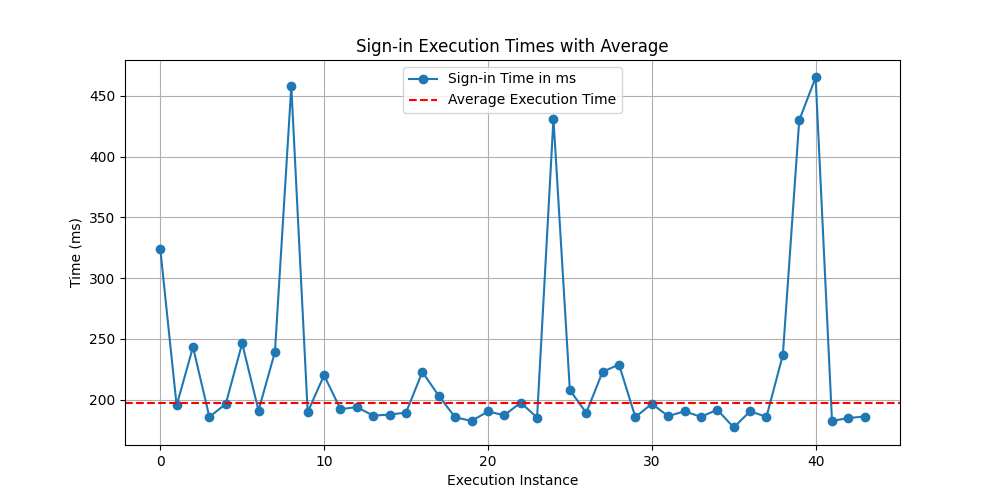
\includegraphics[width=\linewidth]{./imgs/signinTimes.png}
    \caption{Component Diagram}
    \label{fig: High level component diagram}
\end{figure}

As you can see it's clear that we satisfy the non-functional requirement.

\subsubsection{NFR234} Photos captured with the system will be in a quality high
enough to differentiate objects within frame.
\renewcommand{\arraystretch}{1.5}
\begin{center}
  \testcase{
	\textbf{NFST-CM-3} & \textbf{Image Quality Validation}\\\hline

	\textbf{Description} & Test to check if captured image have sufficient quality \\ 

    \textbf{Input} & Captured image of shared space \\ 

    \textbf{Exp. Output} & Image of shared space \\ 

    \textbf{Act. Output} & Image of shared space \\ 
    
	\small \textbf{Evaluation} & Acceptance testing\\    
    
    \small \textbf{Result} & Pass\\ 
  }
\end{center}

\subsubsection{NFR221}
The chatbot shall not disclose any sensitive information in its
messages such as addresses or full names.
\renewcommand{\arraystretch}{1.5}
\begin{center}
  \testcase{
	\textbf{NFST-UAHM-4} & \textbf{Authentication Response Time}\\\hline

	\textbf{Description} & Tests if system authenticates a user within a median response time of under 1 second \\ 

    \textbf{Input} & Correct user login credentials filled in login elements \\ 

    \textbf{Exp. Output} & Authentication process completed within one second \\ 

    \textbf{Act. Output} & Authentication process completed within one second \\ 
    
	\small \textbf{Evaluation} & Acceptance testing\\    
    
    \small \textbf{Result} & Pass\\ 
  }
\end{center}

\subsubsection{NFR235}
The system shall process image data in under 30 minutes.

To test this, we ran the image processing algorithm 100 times on both a high-spec and a low-spec machine and averaged the execution matrix.

The specifications for the low-spec machine are:
\begin{itemize}
\item \textbf{GPU}: Integrated Graphics with CPU (shared GPU memory of 8GB)
\item \textbf{RAM}: 16 GB
\item \textbf{CPU cores}: 6 with 12 logical processors
\item \textbf{CPU speed}: 2.5 GHz

\end{itemize}
The specifications for the high-spec machine are:
\begin{itemize}
\item \textbf{GPU}:  NVIDIA Geforce GTX 1650 (4 GB dedicated GPU memory, 8 GB shared, 12 GB total)
\item \textbf{RAM}: 16 GB
\item \textbf{CPU cores}: 6 with 12 logical processors
\item \textbf{CPU speed}: 4 GHz
\end{itemize}


\begin{figure}[H]
    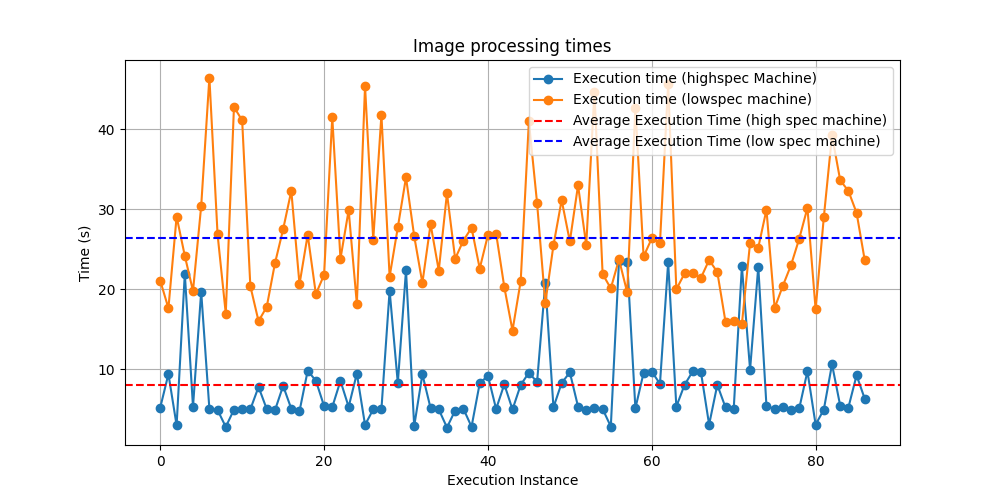
\includegraphics[width=\linewidth]{./imgs/cleanAlgTimes.png}
    \caption{Component Diagram}
    \label{fig: High level component diagram}
\end{figure}

As you can see it's clear that we satisfy the non-functional requirement.

\subsection{Privacy and Security}
\subsubsection{NFR211}
All data related to authentication must be encrypted in both
transit and in storage.
\renewcommand{\arraystretch}{1.5}
\begin{center}
  \testcase{
	\textbf{NFST-UAHM-1} & \textbf{Encryption of Authentication Data}\\\hline

	\textbf{Description} & Tests if system encrypts data in transit and when stored \\ 

    \textbf{Input} & User inputted data in login elements \\ 

    \textbf{Exp. Output} & Stored and data in transit are encrypted \\ 

    \textbf{Act. Output} & Stored and data in transit are encrypted \\ 
    
	\small \textbf{Evaluation} & Acceptance testing\\    
    
    \small \textbf{Result} & Pass\\ 
  }
\end{center}

\subsubsection{NFR212}
Error messages related to authentication should not disclose
sensitive details such as ”Incorrect Password”.
\renewcommand{\arraystretch}{1.5}
\begin{center}
  \testcase{
	\textbf{NFST-UAHM-2} & \textbf{Sensitive Information Error Management}\\\hline

	\textbf{Description} & Tests if the system does not reveal sensitive user information during login attempts \\ 

    \textbf{Input} & Valid email and incorrect password \\ 

    \textbf{Exp. Output} & Error message that avoids revealing sensitive information \\ 

    \textbf{Act. Output} & Error message that avoids revealing sensitive information \\ 
    
	\small \textbf{Evaluation} & Acceptance testing\\    
    
    \small \textbf{Result} & Pass\\ 
  }
\end{center}

\subsubsection{NFR213}
All data related to houses such as addresses and residents should
be encrypted in transit and in rest.
\renewcommand{\arraystretch}{1.5}
\begin{center}
  \testcase{
	\textbf{NFST-UAHM-3} & \textbf{Encryption of House Data}\\\hline

	\textbf{Description} & Tests if system encrypts all data related to houses in transit and at rest \\ 

    \textbf{Input} & View or edit house data \\ 

    \textbf{Exp. Output} & Verification that data in transit and stored data are encrypted \\ 

    \textbf{Act. Output} & Verification that data in transit and stored data are encrypted \\ 
    
	\small \textbf{Evaluation} & Acceptance testing\\    
    
    \small \textbf{Result} & Pass\\ 
  }
\end{center}

\subsubsection{NFR233}
The system shall encrypt and securely store all images of homes.
\renewcommand{\arraystretch}{1.5}
\begin{center}
  \testcase{
	\textbf{NFST-CM-2} & \textbf{Encryption of Images and Videos}\\\hline

	\textbf{Description} & Tests system to ensure encryption and secure storage of images and videos. \\ 

    \textbf{Input} & Captured image and recording of shared space \\ 

    \textbf{Exp. Output} & Image recording in storage are encrypted \\ 

    \textbf{Act. Output} & Image recording in storage are encrypted \\ 
    
	\small \textbf{Evaluation} & Acceptance testing\\    
    
    \small \textbf{Result} & Pass\\ 
  }
\end{center}

\subsubsection{NFR244}
The calendar system shall encrypt all events stored.
\renewcommand{\arraystretch}{1.5}
\begin{center}
  \testcase{
	\textbf{NFST-SC-3} & \textbf{Events Are Encrypted}\\\hline

	\textbf{Description} & Tests if system encrypts stored events \\ 

	\textbf{Input} & Creating event \\ 

    \textbf{Exp. Output} & Event is encrypted in transit and storage \\ 

    \textbf{Act. Output} & Event is encrypted in transit and storage \\ 
    
	\small \textbf{Evaluation} & Acceptance testing\\    
    
    \small \textbf{Result} & Pass\\ 
  }
\end{center}

\subsubsection{NFR251}
The Bill Splitter system shall encrypt all events stored.
\renewcommand{\arraystretch}{1.5}
\begin{center}
  \testcase{
	\textbf{NFST-BSC-1} & \textbf{Events Are Encrypted}\\\hline

	\textbf{Description} & Tests if system encrypts bill splitter events \\ 

	\textbf{Input} & Bill splitting is used \\ 

    \textbf{Exp. Output} & Event is encrypted in transit and storage \\ 

    \textbf{Act. Output} & Event is encrypted in transit and storage \\ 
    
	\small \textbf{Evaluation} & Acceptance testing\\    
    
    \small \textbf{Result} & Pass\\ 
  }
\end{center}

\subsection{Other}
\subsubsection{NFR222}
The chatbot shall not send users too frequently to prevent
annoying users.
\renewcommand{\arraystretch}{1.5}
\begin{center}
  \testcase{
	\textbf{NFST-CC-2} & \textbf{User Messaging Frequency}\\\hline

	\textbf{Description} & Tests ChatBot to ensure it reasonably messages user and not too frequently. \\ 

	\textbf{Input} & Trigger multiple notifications. \\ 

    \textbf{Exp. Output} & Verify notifications are not excessively frequent \\ 

    \textbf{Act. Output} & Verify notifications are not excessively frequent \\ 
    
	\small \textbf{Evaluation} & Acceptance testing\\    
    
    \small \textbf{Result} & Pass\\ 
  }
\end{center}

\subsubsection{NFR236}
The system shall not report false events which accuse someone of
reducing the cleanliness score of an environment.
\renewcommand{\arraystretch}{1.5}
\begin{center}
  \testcase{
	\textbf{NFCT-CM-5} & \textbf{False Event Prevention}\\\hline

	\textbf{Description} & Test to check if system avoids false \\ 

	\textbf{Input} & User uses shared space but does not make a mess. \\ 

    \textbf{Exp. Output} & Objects that were not changed are not listed \\ 

    \textbf{Act. Output} & Objects that were not changed are not listed \\ 
    
	\small \textbf{Evaluation} & Acceptance testing\\    
    
    \small \textbf{Result} & Pass\\ 
  }
\end{center}

\subsubsection{NFR241}
The calendar system shall store all calendar events in UTC.
\renewcommand{\arraystretch}{1.5}
\begin{center}
  \testcase{
	\textbf{NFIT-SC-1} & \textbf{Calendar Event Time Storage and Display}\\\hline

	\textbf{Description} & Tests calendar to ensure event time in database is in UTC but on user's application is displayed in user's local time. \\ 

    \textbf{Input} & Event scheduled with specific time and date. \\ 

    \textbf{Exp. Output} & Event in database in UTC and on user's calendar in their local time \\ 

    \textbf{Act. Output} & Event in database in UTC and on user's calendar in their local time \\ 
    
	\small \textbf{Evaluation} & Acceptance testing\\    
    
    \small \textbf{Result} & Pass\\ 
  }
\end{center}

\subsubsection{NFR243}
The calendar system shall have a granularity of 5 minutes.
\renewcommand{\arraystretch}{1.5}
\begin{center}
  \testcase{
	\textbf{NFIT-SC-1} & \textbf{Calendar Event Time Storage and Display}\\\hline

	\textbf{Description} & Tests calendar to ensure event time in database is in UTC but on user's application is displayed in user's local time. \\ 

    \textbf{Input} & Event scheduled with specific time and date. \\ 

    \textbf{Exp. Output} & Event in database in UTC and on user's calendar in their local time \\ 

    \textbf{Act. Output} & Event in database in UTC and on user's calendar in their local time \\ 
    
	\small \textbf{Evaluation} & Acceptance testing\\    
    
    \small \textbf{Result} & Pass\\ 
  }
\end{center}

\subsubsection{NFR252}
The Bill Splitter shall allow users to record numerical values of
prices with a granularity of two decimal places.
\renewcommand{\arraystretch}{1.5}
\begin{center}
  \testcase{
	\textbf{NFCT-BSC-2} & \textbf{Precision of Numerical Values}\\\hline

	\textbf{Description} & Tests bill splitter's ability to calculate and display numerical values with preicion of two decimal places. \\ 

	\textbf{Input} & Prices entered to split between two users. \\ 

    \textbf{Exp. Output} & Price each user owes is display \\ 

    \textbf{Act. Output} & Price each user owes is display \\ 
    
	\small \textbf{Evaluation} & Acceptance testing\\    
    
    \small \textbf{Result} & Pass\\ 
  }
\end{center}

\section{Unit Testing}
Unit testing for this project is defined as a way of testing the smallest piece of code that can be logically isolated. Logical isolation means to isolate a piece of code based on a particular function. In this project, unit testing was performed on the user-facing application of the project while the other codebases of the project will be tested with other methods.\\\\For context on the this section of the report, the client-facing application was built using the following tools:
\begin{itemize}
\item \textbf{Next.js} as the JavaScript framework for both front-end and back-end
\item \textbf{ReactQuery} for data synchronization and caching
\end{itemize}
and is broken up into different pages based on application features such as:
\begin{itemize}
\item Cleanliness management system
\item Chore scheduling system
\item Bill splitting system
\end{itemize}
While it is recommended to test as much of your code as possible. Due to time constraints and generally better use of our time, the team developed unit tests only for the critical components (Referring to React components) of our application, while other components that exist for purposes such as reusable styling or wrappers were ignoring. In general, unit tests were written with the objective of:
\begin{itemize}
\item Ensure key UI components were rendering
\item Ensuring the UI displayed information fetched from the back-end
\item Ensuring inputs and buttons on the UI are able to be interacted with
\end{itemize}
In the front-end, 115 different tests were written for over 20+ components resulting in the following code-coverage report.


% Define new column types with smaller font
\newcolumntype{S}[1]{>{\small\raggedright\arraybackslash}p{#1}}
\newcolumntype{U}[1]{>{\small\raggedright\arraybackslash}p{#1}}

\newgeometry{left=5mm,right=5mm}
\begin{longtable}{|S{0.3\linewidth} | >{\centering\arraybackslash}p{0.1\linewidth} | >{\centering\arraybackslash}p{0.1\linewidth} | >{\centering\arraybackslash}p{0.1\linewidth} | >{\centering\arraybackslash}p{0.1\linewidth} | U{0.1\linewidth}|}
    \caption{\bf Front-end Code Coverage Report} \label{tab:coverage} \\
      \hline
      \textbf{File} & \textbf{\% Stmts} & \textbf{\% Branch} & \textbf{\% Funcs} & \textbf{\% Lines} & \textbf{Uncovered Line \#s} \\
      \hline
      \endfirsthead
      
      \hline
      \textbf{File} & \textbf{\% Stmts} & \textbf{\% Branch} & \textbf{\% Funcs} & \textbf{\% Lines} & \textbf{Uncovered Line \#s} \\
      \hline
      \endhead
      
      \hline
      \endfoot
      
      \hline
      \endlastfoot

      All files & 83.2 & 91.05 & 58.33 & 83.2 & \\ \hline
      app & 100 & 100 & 100 & 100 & \\ \hline
      \quad page.tsx & 100 & 100 & 100 & 100 & \\ \hline
      app/(main)/bill-splitter/components & 83.37 & 100 & 60 & 83.37 & \\ \hline
      \quad debtsTable.tsx & 83.72 & 100 & 25 & 83.72 & 26--32, 34--38, 76--77 \\ \hline
      \quad historyTable.tsx & 100 & 100 & 100 & 100 & \\ \hline
      \quad loansTable.tsx & 63.82 & 100 & 57.14 & 63.82 & 22--67, 91--93, 95--96 \\ \hline
      \quad summaryCard.tsx & 100 & 100 & 100 & 100 & \\ \hline
      \quad summaryCardStub.tsx & 100 & 100 & 100 & 100 & \\ \hline
      app/(main)/bill-splitter/hooks & 33.33 & 100 & 12.5 & 33.33 & \\ \hline
      \quad patchOwe.ts & 55.26 & 100 & 50 & 55.26 & 5--21 \\ \hline
      \quad useBillHistory.ts & 19.44 & 100 & 0 & 19.44 & 6--29, 32--36 \\ \hline
      \quad useBills.ts & 26.08 & 100 & 0 & 26.08 & 5--16, 19--23 \\ \hline
      \quad useOwes.ts & 26.08 & 100 & 0 & 26.08 & 5--16, 19--23 \\ \hline
      app/(main)/chatbot & 95.62 & 80 & 50 & 95.62 & \\ \hline
      \quad page.tsx & 95.62 & 80 & 50 & 95.62 & 81--85, 101 \\ \hline
      app/(main)/chatbot/components & 95.74 & 33.33 & 50 & 95.74 & \\ \hline
      \quad chatbot-setting-stub.tsx & 95.74 & 33.33 & 50 & 95.74 & 21--22 \\ \hline
      app/(main)/chatbot/hooks & 24.39 & 100 & 0 & 24.39 & \\ \hline
      \quad useActivateChatbot.ts & 24.39 & 100 & 0 & 24.39 & 9--24, 27--41 \\ \hline
      app/(main)/cleanliness-manager/components & 88 & 77.77 & 62.5 & 88 & \\ \hline
      \quad cleanliness-details-modal.tsx & 86.45 & 16.66 & 100 & 86.45 & 39--50, 62 \\ \hline
      \quad cleanliness-image.tsx & 30.76 & 100 & 0 & 30.76 & 11--37 \\ \hline
      \quad cleanliness-logs.tsx & 100 & 100 & 100 & 100 & \\ \hline
      \quad cleanliness-past.tsx & 100 & 100 & 100 & 100 & \\ \hline
      \quad task-card.tsx & 91.8 & 75 & 33.33 & 91.8 & 50, 79--83, 90--93 \\ \hline
      \quad task-list.tsx & 100 & 100 & 100 & 100 & \\ \hline
      app/(main)/cleanliness-manager/hooks & 54.1 & 100 & 20 & 54.1 & \\ \hline
      \quad useCleanlinessLogs.tsx & 46.34 & 100 & 33.33 & 46.34 & 6--27 \\ \hline
      \quad useGetCleanlinessTasks.tsx & 67.85 & 100 & 0 & 67.85 & 37--49, 52--56 \\ \hline
      \quad useUpdateCleanlinessTask.tsx & 44.89 & 100 & 20 & 44.89 & 13--26, 33--34, 36--41, 43--47 \\ \hline
      app/(main)/dashboard/components & 100 & 100 & 100 & 100 & \\ \hline
      \quad dashboard-cards.tsx & 100 & 100 & 100 & 100 & \\ \hline
      app/(main)/house-settings/components & 100 & 100 & 100 & 100 & \\ \hline
      \quad create-note-modal.tsx & 100 & 100 & 100 & 100 & \\ \hline
      \quad edit-house-modal.tsx & 100 & 100 & 100 & 100 & \\ \hline
      \quad house-invites.tsx & 100 & 100 & 100 & 100 & \\ \hline
      \quad house-notes.tsx & 100 & 100 & 100 & 100 & \\ \hline
      \quad invite-user-modal.tsx & 100 & 100 & 100 & 100 & \\ \hline
      app/(main)/house-settings/hooks & 35 & 100 & 20 & 35 & \\ \hline
      \quad useRemoveRoomate.ts & 35 & 100 & 20 & 35 & 5--15, 22--23, 25--32, 34--38 \\ \hline
      app/(main)/profile & 87.22 & 80 & 60 & 87.22 & \\ \hline
      \quad page.tsx & 87.22 & 80 & 60 & 87.22 & 25--31, 39--43, 94--101, 159--161 \\ \hline
      app/(main)/schedule & 23.07 & 100 & 0 & 23.07 & \\ \hline
      \quad adapters.ts & 23.07 & 100 & 0 & 23.07 & 4--13 \\ \hline
      app/(main)/schedule/components & 98.76 & 95.74 & 100 & 98.76 & \\ \hline
      \quad chore-history.tsx & 100 & 100 & 100 & 100 & \\ \hline
      \quad create-chore-modal.tsx & 99.41 & 85.71 & 100 & 99.41 & 143 \\ \hline
      \quad pending-chores.tsx & 100 & 100 & 100 & 100 & \\ \hline
      \quad pending-item.tsx & 100 & 100 & 100 & 100 & \\ \hline
      \quad schedule-item.tsx & 95.58 & 92 & 100 & 95.58 & 64--69, 76--77 \\ \hline
      \quad schedule.tsx & 100 & 100 & 100 & 100 & \\ \hline
      app/(main)/schedule/hooks & 33.48 & 100 & 0 & 33.48 & \\ \hline
      \quad useCreateChore.ts & 14.28 & 100 & 0 & 14.28 & 5--17, 20--42 \\ \hline
      \quad useDeleteChore.ts & 14.63 & 100 & 0 & 14.63 & 5--16, 19--41 \\ \hline
      \quad useGetAllActivities.ts & 36.36 & 100 & 0 & 36.36 & 7--15, 18--22 \\ \hline
      \quad useGetAllCompletedChores.ts & 69.76 & 100 & 0 & 69.76 & 29--36, 39--43 \\ \hline
      \quad useGetCompletedChores.ts & 50 & 100 & 0 & 50 & 12--19, 22--26 \\ \hline
      \quad useUpdateCompletedChore.ts & 24 & 100 & 0 & 24 & 11--23, 26--50 \\ \hline
      app/auth/hooks & 47.36 & 100 & 0 & 47.36 & \\ \hline
      \quad useUser.tsx & 47.36 & 100 & 0 & 47.36 & 19--38 \\ \hline
      components & 100 & 100 & 85.71 & 100 & \\ \hline
      \quad loading.tsx & 100 & 100 & 100 & 100 & \\ \hline
      \quad modal.tsx & 100 & 100 & 100 & 100 & \\ \hline
      \quad mutate-loading.tsx & 100 & 100 & 100 & 100 & \\ \hline
      \quad query-provider.tsx & 100 & 100 & 100 & 100 & \\ \hline
      \quad roommates-table.tsx & 100 & 100 & 50 & 100 & \\ \hline
      components/ui & 98.1 & 88.88 & 100 & 98.1 & \\ \hline
      \quad badge.tsx & 100 & 100 & 100 & 100 & \\ \hline
      \quad button.tsx & 100 & 50 & 100 & 100 & 42 \\ \hline
      \quad card.tsx & 100 & 100 & 100 & 100 & \\ \hline
      \quad checkbox.tsx & 100 & 100 & 100 & 100 & \\ \hline
      \quad dialog.tsx & 100 & 100 & 100 & 100 & \\ \hline
      \quad form.tsx & 92.26 & 92.85 & 100 & 92.26 & 50--51, 123--133 \\ \hline
      \quad input.tsx & 100 & 100 & 100 & 100 & \\ \hline
      \quad label.tsx & 100 & 100 & 100 & 100 & \\ \hline
      \quad popover.tsx & 100 & 100 & 100 & 100 & \\ \hline
      \quad switch.tsx & 100 & 100 & 100 & 100 & \\ \hline
      \quad table.tsx & 100 & 100 & 100 & 100 & \\ \hline
      \quad tabs.tsx & 100 & 100 & 100 & 100 & \\ \hline
      hooks & 50 & 69.23 & 53.84 & 50 & \\ \hline
      \quad useGetHouse.ts & 65.51 & 60 & 100 & 65.51 & 10--19 \\ \hline
      \quad useRoommates.ts & 63.33 & 60 & 100 & 63.33 & 9--11, 13--20 \\ \hline
      \quad useToast.ts & 45.5 & 100 & 14.28 & 45.5 & 27--30, 59--72, 75--125, 131--136, 140--167 \\ \hline
      lib & 61.53 & 100 & 50 & 61.53 & \\ \hline
      \quad utils.ts & 61.53 & 100 & 50 & 61.53 & 9--13 \\ \hline
      lib/constants & 100 & 100 & 100 & 100 & \\ \hline
      \quad index.ts & 100 & 100 & 100 & 100 & \\ \hline
      lib/supabase & 44.44 & 100 & 0 & 44.44 & \\ \hline
      \quad browser.ts & 44.44 & 100 & 0 & 44.44 & 5--9 \\ \hline

\end{longtable}
\restoregeometry

\section{Functional Testing}
Functional testing is described as ensuring that the system behaves as expected given specific inputs. In the case of Room8, the functional testing is implemented in the form of 

\newgeometry{left=5mm,right=5mm}
\begin{longtable}{|S{0.3\linewidth} | >{\centering\arraybackslash}p{0.1\linewidth} | >{\centering\arraybackslash}p{0.1\linewidth} | >{\centering\arraybackslash}p{0.1\linewidth} | U{0.1\linewidth}|}
    \caption{\bf Detector Code Coverage Report} \label{tab:coverage} \\
      \hline
      \textbf{File} & \textbf{\% Stmts} & \textbf{\% Miss} & \textbf{\% Cover} & \textbf{Missing} \\
      \hline
      \endfirsthead
      
      \hline
      \textbf{File} & \textbf{\% Stmts} & \textbf{\% Miss} & \textbf{\% Cover} & \textbf{Missing} \\
      \hline
      \endhead
      
      \hline
      \endfoot
      
      \hline
      \endlastfoot

      main.py & 300 & 129 & 57 & 63, 96, 138-140, 193-207, 238, 248, 289, 339-396, 401-469, 474-519, 522-545 \\ \hline
      testCleanlinessDetector.py & 29 & 0 & 100 & \\ \hline
      TOTAL & 329 & 129 & 61 & \\ \hline

\end{longtable}
\restoregeometry

\section{Changes Due to Testing}
\textbf{FR211} - Change description to use Google account instead of using name, email and password.\\
\textbf{FST-UAHM-1} - See above description. \\
\textbf{FST-UAHM-2} - Change input field of test case to using Google account instead of email and password. \\
\textbf{FST-CM-1} - Changed description to remove cleanliness score and add listing objects chaged. \\
\textbf{FR232} - Removing because of it is no longer part of the implementation scope. \\
\textbf{FST-CM-2} - Editing test case to remove cleanliness score mentions and update to showing after images. \\
\textbf{NFR236} - Removing mention of cleanliness score. \\
\textbf{NFCT-CM-5} - See above description. \\



\subsection{Changes Due to Unit Testing}
Unit testing discovered several bugs and anti-patterns in the front-end codebase that were resolved. Some examples of the discovered flaws include:
\begin{itemize}
\item Invalid references for form inputs and form labels. Leading to input labels not focusing their corresponding form input.
\item Unneccessary props on React components.
\item Missing semantic HTML attributes such as "role" on various items. Making the app less accessible and more difficult for the testing library to find components.
\item Checking for lists to be empty with <LIST VARIABLE NAME>. This resulted in empty lists still being evaluated to "True" because in JS empty lists are truthy and resulted in code logic that was supposed to trigger when the list was empty to not work as expected.
\item Displaying times without the timezone. This was detected because the testing suite failed on various environments due to the timezone printing differently on machines with different timezones.
\end{itemize}
The code coverage reports shows some trends, mainly that all most if not all of our hooks have poor code coverage rates. This is expected and acceptable because the purpose of the hooks is to fetch data from the back-end and display it on the front-end and since we were mocking the back-end data, most of the hooks' functionality were not used.

\section{Automated Testing}
Automated tests include the unit tests and the cleanliness detection system's test samples. The front-end tests were additionally automated to run on push and on merge requests to main and dev. These automated tests on GitHub in conjunction with branch rules that prevent merging branches which fail tests ensure that no changes the fail tests will make it to the production environment.
		
\section{Trace to Requirements}
    \begin{itemize}
      \item \textbf{FR211:} FST-UAHM-1
      \item \textbf{FR212:} FST-UAHM-2
      \item \textbf{FR213:} FST-UAHM-3
      \item \textbf{FR214:} FST-UAHM-4
      \item \textbf{FR215:} FST-UAHM-5
      \item \textbf{FR216:} FST-UAHM-4
      \item \textbf{FR217:} FST-UAHM-5
      \item \textbf{FR218:} FST-UAHM-5, FST-UAHM-6
      \item \textbf{FR221:} FST-CC-1
      \item \textbf{FR222:} FST-CC-3
      \item \textbf{FR223:} FST-CC-3
      \item \textbf{FR224:} FST-CC-3
      \item \textbf{FR231:} FST-CM-1
      \item \textbf{FR233:} FST-CM-2
      \item \textbf{FR234:} FST-CM-2
      \item \textbf{FR235:} FST-CM-2
      \item \textbf{FR241:} FST-SC-1
      \item \textbf{FR242:} FST-SC-1
      \item \textbf{FR243:} FST-SC-1
      \item \textbf{FR244:} FST-SC-2, FST-SC-3
      \item \textbf{FR245:} FST-SC-1, FST-SC-4
      \item \textbf{FR251:} FST-BSC-1
      \item \textbf{FR252:} FST-BSC-2
      \item \textbf{FR253:} FST-BSC-2, FST-BSC-3
      \item \textbf{FR254:} FST-BSC-3
      \item \textbf{FR255:} FST-BSC-1
    \end{itemize}

\section{Trace to Modules}
\renewcommand{\arraystretch}{1.5}
\begin{center}
  \begin{tabular}{|p{5cm}|p{10cm}|}
    \hline
    \textbf{Module} & \textbf{Tests} \\
    \hline
    \textbf{Account Management} &  FST-UAHM-1, FST-UAHM-2, FST-UAHM-3, FST-UAHM-4, NFST-UAHM-1, NFST-UAHM-2\\ 
    \hline
    \textbf{Home Management} & FST-UAHM-4, FST-UAHM-5, FST-UAHM-6, NFST-UAHM-3\\ 
    \hline
    \textbf{Schedule Manager} &  FST-SC-1, FST-SC-2, FST-SC-3, FST-SC-1, FST-SC-4, NFIT-SC-1, NFST-SC-3, NFIT-SC-1 \\ 
    \hline
    \textbf{Bill Splitter} & FST-BSC-1, FST-BSC-2, FST-BSC-3, NFST-BSC-1, NFCT-BSC-2 \\ 
    \hline
    \textbf{Cleanliness Manager} & FST-CM-1, FST-CM-2, NFST-CM-6, NFST-CM-3, NFST-CM-2, NFCT-CM-5\\    
    \hline
    \textbf{SMS ChatBot} & FST-CC-1, FST-CC-3, NFST-CC-2\\ 
    \hline
  \end{tabular}
\end{center}


\section{Code Coverage Metrics}
\newgeometry{left=5mm,right=5mm}
\setcounter{table}{0}
\begin{longtable}{|S{0.3\linewidth} | >{\centering\arraybackslash}p{0.1\linewidth} | >{\centering\arraybackslash}p{0.1\linewidth} | >{\centering\arraybackslash}p{0.1\linewidth} | >{\centering\arraybackslash}p{0.1\linewidth} | U{0.1\linewidth}|}
    \caption{\bf Front-end Code Coverage Report} \label{tab:coverage} \\
      \hline
      \textbf{File} & \textbf{\% Stmts} & \textbf{\% Branch} & \textbf{\% Funcs} & \textbf{\% Lines} & \textbf{Uncovered Line \#s} \\
      \hline
      \endfirsthead
      
      \hline
      \textbf{File} & \textbf{\% Stmts} & \textbf{\% Branch} & \textbf{\% Funcs} & \textbf{\% Lines} & \textbf{Uncovered Line \#s} \\
      \hline
      \endhead
      
      \hline
      \endfoot
      
      \hline
      \endlastfoot

      All files & 83.2 & 91.05 & 58.33 & 83.2 & \\ \hline
      app & 100 & 100 & 100 & 100 & \\ \hline
      \quad page.tsx & 100 & 100 & 100 & 100 & \\ \hline
      app/(main)/bill-splitter/components & 83.37 & 100 & 60 & 83.37 & \\ \hline
      \quad debtsTable.tsx & 83.72 & 100 & 25 & 83.72 & 26--32, 34--38, 76--77 \\ \hline
      \quad historyTable.tsx & 100 & 100 & 100 & 100 & \\ \hline
      \quad loansTable.tsx & 63.82 & 100 & 57.14 & 63.82 & 22--67, 91--93, 95--96 \\ \hline
      \quad summaryCard.tsx & 100 & 100 & 100 & 100 & \\ \hline
      \quad summaryCardStub.tsx & 100 & 100 & 100 & 100 & \\ \hline
      app/(main)/bill-splitter/hooks & 33.33 & 100 & 12.5 & 33.33 & \\ \hline
      \quad patchOwe.ts & 55.26 & 100 & 50 & 55.26 & 5--21 \\ \hline
      \quad useBillHistory.ts & 19.44 & 100 & 0 & 19.44 & 6--29, 32--36 \\ \hline
      \quad useBills.ts & 26.08 & 100 & 0 & 26.08 & 5--16, 19--23 \\ \hline
      \quad useOwes.ts & 26.08 & 100 & 0 & 26.08 & 5--16, 19--23 \\ \hline
      app/(main)/chatbot & 95.62 & 80 & 50 & 95.62 & \\ \hline
      \quad page.tsx & 95.62 & 80 & 50 & 95.62 & 81--85, 101 \\ \hline
      app/(main)/chatbot/components & 95.74 & 33.33 & 50 & 95.74 & \\ \hline
      \quad chatbot-setting-stub.tsx & 95.74 & 33.33 & 50 & 95.74 & 21--22 \\ \hline
      app/(main)/chatbot/hooks & 24.39 & 100 & 0 & 24.39 & \\ \hline
      \quad useActivateChatbot.ts & 24.39 & 100 & 0 & 24.39 & 9--24, 27--41 \\ \hline
      app/(main)/cleanliness-manager/components & 88 & 77.77 & 62.5 & 88 & \\ \hline
      \quad cleanliness-details-modal.tsx & 86.45 & 16.66 & 100 & 86.45 & 39--50, 62 \\ \hline
      \quad cleanliness-image.tsx & 30.76 & 100 & 0 & 30.76 & 11--37 \\ \hline
      \quad cleanliness-logs.tsx & 100 & 100 & 100 & 100 & \\ \hline
      \quad cleanliness-past.tsx & 100 & 100 & 100 & 100 & \\ \hline
      \quad task-card.tsx & 91.8 & 75 & 33.33 & 91.8 & 50, 79--83, 90--93 \\ \hline
      \quad task-list.tsx & 100 & 100 & 100 & 100 & \\ \hline
      app/(main)/cleanliness-manager/hooks & 54.1 & 100 & 20 & 54.1 & \\ \hline
      \quad useCleanlinessLogs.tsx & 46.34 & 100 & 33.33 & 46.34 & 6--27 \\ \hline
      \quad useGetCleanlinessTasks.tsx & 67.85 & 100 & 0 & 67.85 & 37--49, 52--56 \\ \hline
      \quad useUpdateCleanlinessTask.tsx & 44.89 & 100 & 20 & 44.89 & 13--26, 33--34, 36--41, 43--47 \\ \hline
      app/(main)/dashboard/components & 100 & 100 & 100 & 100 & \\ \hline
      \quad dashboard-cards.tsx & 100 & 100 & 100 & 100 & \\ \hline
      app/(main)/house-settings/components & 100 & 100 & 100 & 100 & \\ \hline
      \quad create-note-modal.tsx & 100 & 100 & 100 & 100 & \\ \hline
      \quad edit-house-modal.tsx & 100 & 100 & 100 & 100 & \\ \hline
      \quad house-invites.tsx & 100 & 100 & 100 & 100 & \\ \hline
      \quad house-notes.tsx & 100 & 100 & 100 & 100 & \\ \hline
      \quad invite-user-modal.tsx & 100 & 100 & 100 & 100 & \\ \hline
      app/(main)/house-settings/hooks & 35 & 100 & 20 & 35 & \\ \hline
      \quad useRemoveRoomate.ts & 35 & 100 & 20 & 35 & 5--15, 22--23, 25--32, 34--38 \\ \hline
      app/(main)/profile & 87.22 & 80 & 60 & 87.22 & \\ \hline
      \quad page.tsx & 87.22 & 80 & 60 & 87.22 & 25--31, 39--43, 94--101, 159--161 \\ \hline
      app/(main)/schedule & 23.07 & 100 & 0 & 23.07 & \\ \hline
      \quad adapters.ts & 23.07 & 100 & 0 & 23.07 & 4--13 \\ \hline
      app/(main)/schedule/components & 98.76 & 95.74 & 100 & 98.76 & \\ \hline
      \quad chore-history.tsx & 100 & 100 & 100 & 100 & \\ \hline
      \quad create-chore-modal.tsx & 99.41 & 85.71 & 100 & 99.41 & 143 \\ \hline
      \quad pending-chores.tsx & 100 & 100 & 100 & 100 & \\ \hline
      \quad pending-item.tsx & 100 & 100 & 100 & 100 & \\ \hline
      \quad schedule-item.tsx & 95.58 & 92 & 100 & 95.58 & 64--69, 76--77 \\ \hline
      \quad schedule.tsx & 100 & 100 & 100 & 100 & \\ \hline
      app/(main)/schedule/hooks & 33.48 & 100 & 0 & 33.48 & \\ \hline
      \quad useCreateChore.ts & 14.28 & 100 & 0 & 14.28 & 5--17, 20--42 \\ \hline
      \quad useDeleteChore.ts & 14.63 & 100 & 0 & 14.63 & 5--16, 19--41 \\ \hline
      \quad useGetAllActivities.ts & 36.36 & 100 & 0 & 36.36 & 7--15, 18--22 \\ \hline
      \quad useGetAllCompletedChores.ts & 69.76 & 100 & 0 & 69.76 & 29--36, 39--43 \\ \hline
      \quad useGetCompletedChores.ts & 50 & 100 & 0 & 50 & 12--19, 22--26 \\ \hline
      \quad useUpdateCompletedChore.ts & 24 & 100 & 0 & 24 & 11--23, 26--50 \\ \hline
      app/auth/hooks & 47.36 & 100 & 0 & 47.36 & \\ \hline
      \quad useUser.tsx & 47.36 & 100 & 0 & 47.36 & 19--38 \\ \hline
      components & 100 & 100 & 85.71 & 100 & \\ \hline
      \quad loading.tsx & 100 & 100 & 100 & 100 & \\ \hline
      \quad modal.tsx & 100 & 100 & 100 & 100 & \\ \hline
      \quad mutate-loading.tsx & 100 & 100 & 100 & 100 & \\ \hline
      \quad query-provider.tsx & 100 & 100 & 100 & 100 & \\ \hline
      \quad roommates-table.tsx & 100 & 100 & 50 & 100 & \\ \hline
      components/ui & 98.1 & 88.88 & 100 & 98.1 & \\ \hline
      \quad badge.tsx & 100 & 100 & 100 & 100 & \\ \hline
      \quad button.tsx & 100 & 50 & 100 & 100 & 42 \\ \hline
      \quad card.tsx & 100 & 100 & 100 & 100 & \\ \hline
      \quad checkbox.tsx & 100 & 100 & 100 & 100 & \\ \hline
      \quad dialog.tsx & 100 & 100 & 100 & 100 & \\ \hline
      \quad form.tsx & 92.26 & 92.85 & 100 & 92.26 & 50--51, 123--133 \\ \hline
      \quad input.tsx & 100 & 100 & 100 & 100 & \\ \hline
      \quad label.tsx & 100 & 100 & 100 & 100 & \\ \hline
      \quad popover.tsx & 100 & 100 & 100 & 100 & \\ \hline
      \quad switch.tsx & 100 & 100 & 100 & 100 & \\ \hline
      \quad table.tsx & 100 & 100 & 100 & 100 & \\ \hline
      \quad tabs.tsx & 100 & 100 & 100 & 100 & \\ \hline
      hooks & 50 & 69.23 & 53.84 & 50 & \\ \hline
      \quad useGetHouse.ts & 65.51 & 60 & 100 & 65.51 & 10--19 \\ \hline
      \quad useRoommates.ts & 63.33 & 60 & 100 & 63.33 & 9--11, 13--20 \\ \hline
      \quad useToast.ts & 45.5 & 100 & 14.28 & 45.5 & 27--30, 59--72, 75--125, 131--136, 140--167 \\ \hline
      lib & 61.53 & 100 & 50 & 61.53 & \\ \hline
      \quad utils.ts & 61.53 & 100 & 50 & 61.53 & 9--13 \\ \hline
      lib/constants & 100 & 100 & 100 & 100 & \\ \hline
      \quad index.ts & 100 & 100 & 100 & 100 & \\ \hline
      lib/supabase & 44.44 & 100 & 0 & 44.44 & \\ \hline
      \quad browser.ts & 44.44 & 100 & 0 & 44.44 & 5--9 \\ \hline

\end{longtable}
\restoregeometry

\begin{longtable}{|S{0.3\linewidth} | >{\centering\arraybackslash}p{0.1\linewidth} | >{\centering\arraybackslash}p{0.1\linewidth} | >{\centering\arraybackslash}p{0.1\linewidth} | U{0.1\linewidth}|}
    \caption{\bf Detector Code Coverage Report} \label{tab:coverage} \\
      \hline
      \textbf{File} & \textbf{\% Stmts} & \textbf{\% Miss} & \textbf{\% Cover} & \textbf{Missing} \\
      \hline
      \endfirsthead
      
      \hline
      \textbf{File} & \textbf{\% Stmts} & \textbf{\% Miss} & \textbf{\% Cover} & \textbf{Missing} \\
      \hline
      \endhead
      
      \hline
      \endfoot
      
      \hline
      \endlastfoot

      main.py & 300 & 129 & 57 & 63, 96, 138-140, 193-207, 238, 248, 289, 339-396, 401-469, 474-519, 522-545 \\ \hline
      testCleanlinessDetector.py & 29 & 0 & 100 & \\ \hline
      TOTAL & 329 & 129 & 61 & \\ \hline

\end{longtable}
\restoregeometry

\bibliographystyle{plainnat}
\bibliography{../../refs/References}

\newpage{}
\section*{Appendix --- Reflection}

The information in this section will be used to evaluate the team members on the
graduate attribute of Reflection.

\input{../Reflection.tex}

\begin{enumerate}
  \item What went well while writing this deliverable? 
  \item What pain points did you experience during this deliverable, and how
    did you resolve them?
  \item Which parts of this document stemmed from speaking to your client(s) or
  a proxy (e.g. your peers)? Which ones were not, and why?
  \item In what ways was the Verification and Validation (VnV) Plan different
  from the activities that were actually conducted for VnV?  If there were
  differences, what changes required the modification in the plan?  Why did
  these changes occur?  Would you be able to anticipate these changes in future
  projects?  If there weren't any differences, how was your team able to clearly
  predict a feasible amount of effort and the right tasks needed to build the
  evidence that demonstrates the required quality?  (It is expected that most
  teams will have had to deviate from their original VnV Plan.)
\end{enumerate}

Answers:
\begin{enumerate}
  \item Compiling results from tests such as code coverage metrics and satisfaction criteria was simple and easy to port over to the document. Additionally, due to how advanced the average testing library is, writing test cases to check various things such as running time, output results, etc is very easy and that made working on the tests for this deliverable very easy. Finally, division of labour in the deliverable was a lot easier because multiple people can contribute to a section independently because our project is divided into separate mini-projects that can each have their own automated tests, unit tests, etc.
  \item Creating appropriate unit tests was difficult at first because the team was inexperienced with writing quality unit tests. After that another pain point that we encountered while writing this document was finding appropriate sections to place our tests for the AI cleanliness detection system. Those tests are neither automated nor are they unit tests but they are extremely relevant. In the end we ended up creating a section for those tests.
  \item Tests for the cleanliness detection system (the AI system) were inspired from conversations with our supervisor Dr. Tharmarasa, who advised us to curate sample cases to prove our system's functionality. Unit tests and generally all front-end tests we're implemented without discussions from users or peers. The reason clients and proxies were not consulted for the development of tests was because our requirements were not built from user feedback.
  \item Our original VnV plan differed from the actual verification and validation activities in several ways. First, the testing tools we used provided unexpected insights into code improvements, such as missing accessibility labels and code smells we hadn't anticipated detecting. Second, some non-functional requirements weren't defined precisely enough to create clear test cases for them, requiring us to develop more specific interpretations. Finally, after completing this VnV report, we gained a much better understanding of what makes a requirement feasibly testable, knowledge we will apply when writing requirements for future projects. These deviations were primarily due to our team's inexperience with comprehensive testing methodologies at the project's outset.
\end{enumerate}

\end{document}
